\subsection{Criteria for surjectivity}

PROPOSITION 4. --- Let E and F be two Fréchet spaces, and u a continuous linear mapping from E into F. The following conditions are equivalent :

\begin{enumerate}
\def\labelenumi{(\roman{enumi})}
\item
  u is surjective.
\item
  For every semi-norm \(p \in \mathbf{S}(\mathbf{E})\) , there exists \(q \in \mathbf{S}(\mathbf{F})\) such that we have \(|f| \leqslant q\) for every linear form \(f \in \mathbf{F}'\) satisfying \(|f \circ u| \leqslant p\) .
\item
  For every semi-norm \(p \in \mathrm{S}(\mathrm{E})\) , there exists \(q \in \mathrm{S}(\mathrm{F})\) satisfying the following property: if a linear form \(f \in F'\) satisfies \(|f \circ u| \leqslant p\) , then f is null on points where q is null and for all \(y \in F\) , \(r \in \mathrm{S}(\mathrm{F})\) , there exists \(x \in E\) with \(r(u(x) - y) = 0\) .
\item
  For every semi-norm \(p \in \mathrm{S}(\mathrm{E})\) , we have
\end{enumerate}

\[
\sup_{\substack{f\in \mathbf{F}^{\prime}\\ |f\circ u|\leqslant p}}\big|f(y)\big| <   + \infty \quad \text{for all} \quad y\in \mathbf{F}  .\tag{1}
\]

We shall prove the proposition according to the following logical scheme

\pandocbounded{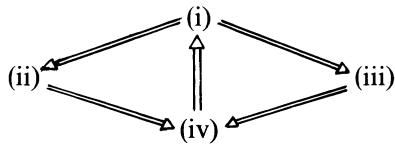
\includegraphics[keepaspectratio]{images/part002_fd83f186.jpg}}

If \(u\) is surjective, it is a strict morphism (IV, p.~28, th. 1) then for every semi-norm \(p \in \mathrm{S}(\mathrm{E})\) , there exists a semi-norm \(q \in \mathrm{S}(\mathrm{F})\) such that, for all \(y \in \mathrm{F}\) satisfying \(q(y) \leqslant 1\) , there exists \(x \in \mathrm{E}\) satisfying \(p(x) \leqslant 1\) and \(u(x) = y\) . We deduce immediately that (i) implies (ii) and (iii). It is clear that (ii) implies (iv).

To prove that (iii) implies (iv), let \(p\) and \(q\) be as in (iii). Let \(y \in \mathbf{F}\) , by (iii), there exists \(x\) in \(\mathbf{E}\) such that \(q(u(x) - y) = 0\) . If \(f \in \mathbf{F}'\) satisfies \(|f \circ u| \leqslant p\) , then we have \(f(u(x) - y) = 0\) , hence

\[
\left| f (y) \right| = \left| f (u (x)) \right| \leqslant p (x)
\]

and the relation (1) is satisfied.

Finally we prove that (iv) implies (i). Let \(p \in \mathrm{S}(\mathrm{E})\) and let \(q\) be the superior envelope of the functions \(|f|\) for \(f \in \mathrm{F}'\) satisfying \(|f \circ u| \leqslant p\) . By (iv), \(q\) is finite on \(\mathrm{F}\) , and is evidently a lower semi-continuous semi-norm on \(\mathrm{F}\) ; since \(\mathrm{F}\) is barrelled (III, p.~25, corollary), we have \(q \in \mathrm{S}(\mathrm{F})\) . Let \(\mathbf{B}_p\) (resp. \(\mathbf{B}_q\) ) denote the set of all \(x \in \mathrm{E}\) (resp. \(y \in \mathrm{F}\) ) such that \(p(x) \leqslant 1\) (resp. \(q(y) \leqslant 1\) ). We have \(q \circ u \leqslant p\) , and so \(u(\mathbf{B}_p) \subset \mathbf{B}_q\) . The polar of \(u(\mathbf{B}_p)\) in \(\mathrm{F}'\) consists of linear forms \(f \in \mathrm{F}'\) such that \(|f \circ u| \leqslant p\) , hence \(|f| \leqslant q\) ; in other words, we get \(u(\mathbf{B}_p)^{\circ} \subset \mathbf{B}_q^{\circ}\) , and finally that \(\overline{u(\mathbf{B}_p)} = \mathbf{B}_q\) follows from the theorem of bipolars (II, p.~45, cor. 3). If \(\mathrm{U}\) is a neighbourhood of 0 in \(\mathrm{E}\) , there exists \(p \in \mathrm{S}(\mathrm{E})\) such that \(\mathbf{B}_p \subset \mathbf{U}\) , hence \(\overline{u(\mathbf{U})}\) contains the neighbourhood \(\mathbf{B}_q\) of 0 in \(\mathrm{F}\) . This implies that \(u\) is surjective (I, p.~17, th. 1).

COROLLARY. --- Suppose E and F are Banach spaces. The following conditions are equivalent :

\begin{enumerate}
\def\labelenumi{(\roman{enumi})}
\item
  \(u\) is surjective.
\item
  There exists a real number \(r > 0\) , such that \(\| f \| \leqslant r\) . \(\| {}^t u(f) \|\) for all \(f \in \mathbf{F}'\) .
\item
  For all \(y \in F\) , we have \(\sup_{\substack{f\in \mathbf{F}^{\prime}\\ |f\circ u|\leqslant 1}} |f(y)| < +\infty\) .
\end{enumerate}

The conditions (ii) and (iii) are in fact reformulations of conditions (ii) and (iv) of prop. 4 for Banach spaces.

